\newpage
\subsection{Method Signatures}
\visHeader
\hypertarget{static:methods vis}{}

To finish defining our types, lets define the \emph{signatures} of some operations they'll eventually support.

\begin{enumerate}
  
\item[$\blacktriangleright$] Right-click \texttt{Partition} to invoke the context-menu as depicted in Fig.~\ref{fig:add_operation}

\item[$\blacktriangleright$] Select \texttt{Partition} and either right-click to invoke the context-menu (Fig.~\ref{fig:add_operation})  and choose ``Features \&
Properties/Operations..'' or simply press \texttt{F10}.

\begin{figure}[htbp]
	\centering
  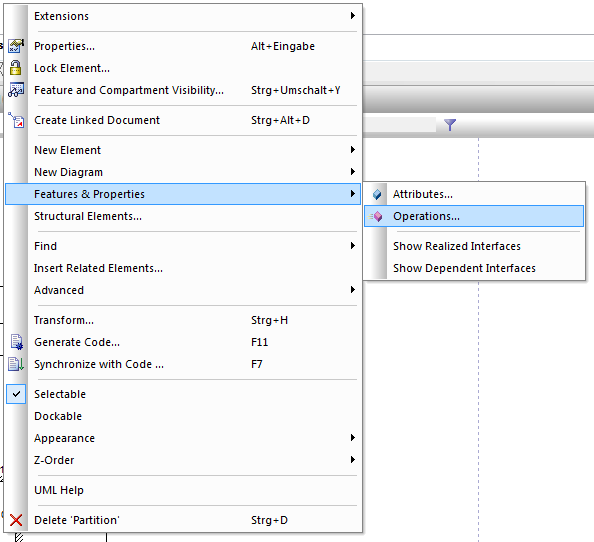
\includegraphics[width=0.8\textwidth]{ea_contextAddOperation}
	\caption{Add an operation}
	\label{fig:add_operation}
\end{figure}
\FloatBarrier

\item[$\blacktriangleright$] In the dialogue that pops-up (Fig.~\ref{fig:operation_properties}), enter `empty' as the \texttt{Name} of the operation,
leave the \texttt{Return Type} as `void', and press \texttt{Save}. 

\vspace{0.5cm}

\item[$\blacktriangleright$] In the same dialogue, press \texttt{New} to add a second operation, \texttt{removeCard}, and edit the values as seen in 
Fig.~\ref{fig:operation_parameters}. Notice that the \texttt{Return Type} can be chosen by either the drop-down menu for
primitives (e.g. \texttt{EBoolean}), or via the `\texttt{\ldots}' button (highlighted in Fig.~\ref{fig:operation_properties}) for types you've established in
the metamodel (e.g. \texttt{Card}).
\vspace{-.3cm}
\begin{quote}
{ \small
$\textbf{Please note:}$ Non-primitive types \emph{must} be chosen via the `\texttt{\ldots}' button. It allows you to browse for the corresponding elements in
your project. Simply typing them won't work!
}
\end{quote}

\begin{figure}[htbp]
	\centering
  	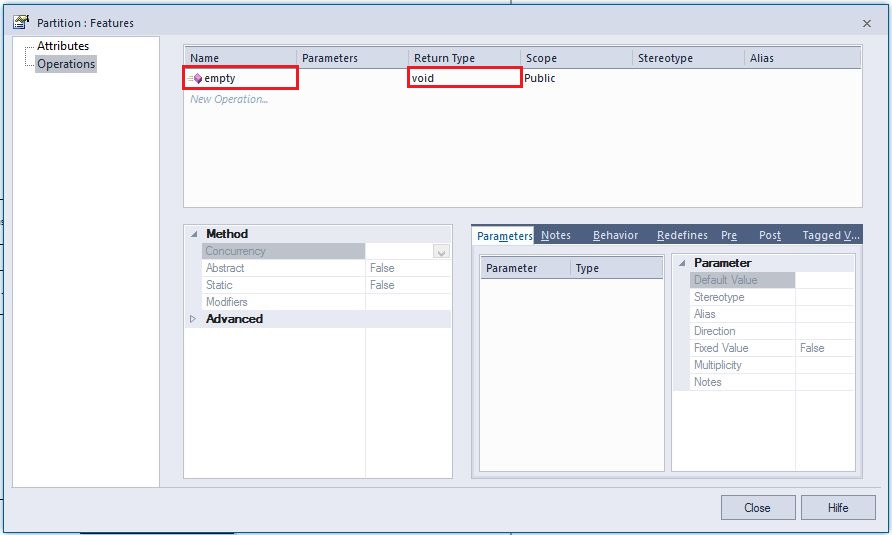
\includegraphics[width=0.8\textwidth]{ea_operationEmpty}
	\caption{EClass properties editor}
	\label{fig:operation_properties}
\end{figure}

\begin{figure}[htbp]
	\centering
  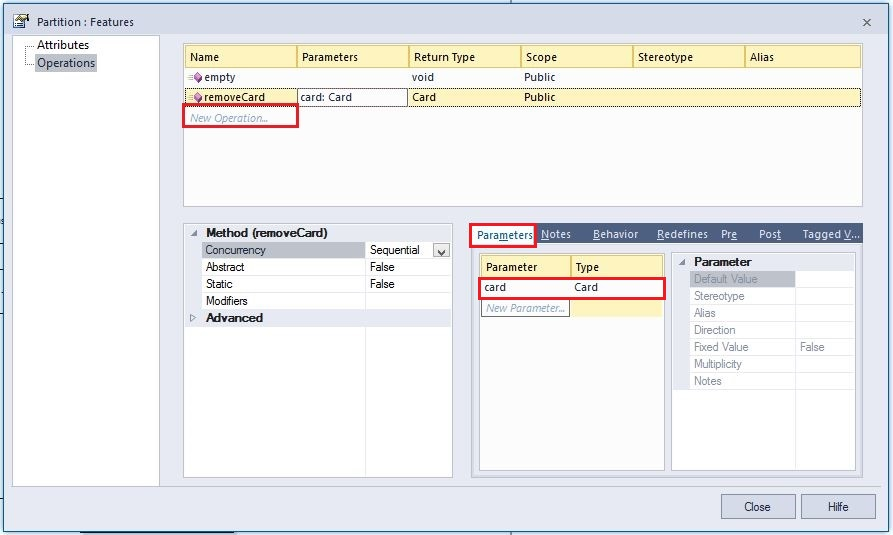
\includegraphics[width=0.85\textwidth]{ea_operationRemoveCard}
	\caption{Parameters and return type}
	\label{fig:operation_parameters}
\end{figure}

\item[$\blacktriangleright$] Parameters can be added by pressing \texttt{Edit}\footnote{You must save the operation before this option will become active} and
completing the dialouge. {\bf \small see Geza comments; mention typing will fail validation here. (use options)}

\item[$\blacktriangleright$] Repeat this process for the \texttt{check} operation (with two parameters), as depicted in Fig.~\ref{fig:operation_partition}. 

\item[$\blacktriangleright$] If you've done everything right, your dialogue should now contain three methods - \texttt{check}, \texttt{empty}, and
\texttt{removeCard} - each with the corresponding parameters and return types in Fig.~\ref{fig:operation_partition}.

\begin{figure}[htbp]
	\centering
  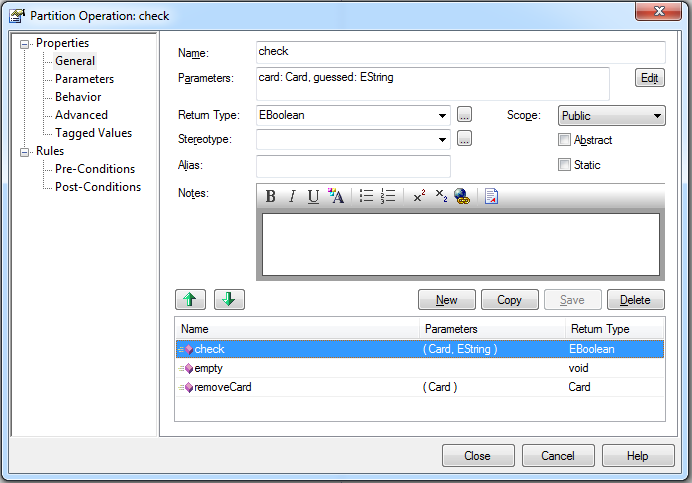
\includegraphics[width=0.9\textwidth]{ea_operationCheck}
	\caption{All operations in \texttt{Partition}}
	\label{fig:operation_partition}
\end{figure}

\item[$\blacktriangleright$] Add all operations analogously for \texttt{Box} and \texttt{Card} so that your metamodel closely resembles
Fig.~\ref{fig:metamodel_complete}.\footnote{Please note that names of parameters may not be displayed by default in EA}

\item[$\blacktriangleright$] To finish, export the metamodel for code generation in Eclipse, and examine the model once again. Each signature should have
appeared in their respective EClass.

\begin{figure}[htbp]
	\centering
  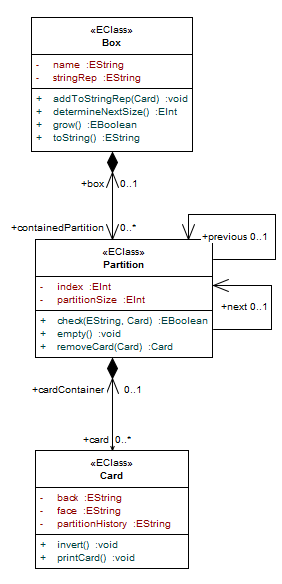
\includegraphics[width=0.63\textwidth]{ea_metamodelComplete.png}
\caption[Complete metamodel for our learning box.]{Complete metamodel for our learning box}
	\label{fig:metamodel_complete}
\end{figure}

\item[$\blacktriangleright$] To see how this complete metamodel is represented in the textual syntax, examine Fig.~\ref{fig:workspaceMethods} in the following
section. 

\end{enumerate}

\fancyfoot[R]{$\triangleright$ \hyperlink{validation vis}{Next}}
